\subsection{Custo do Ataque}

Somente o peso do custo do ataque foi alterado para $5000$.  Os resultados no
planejamento são apresentados na Figura~\ref{fig:atack_5000}.

\begin{figure}[H]
  \centering
  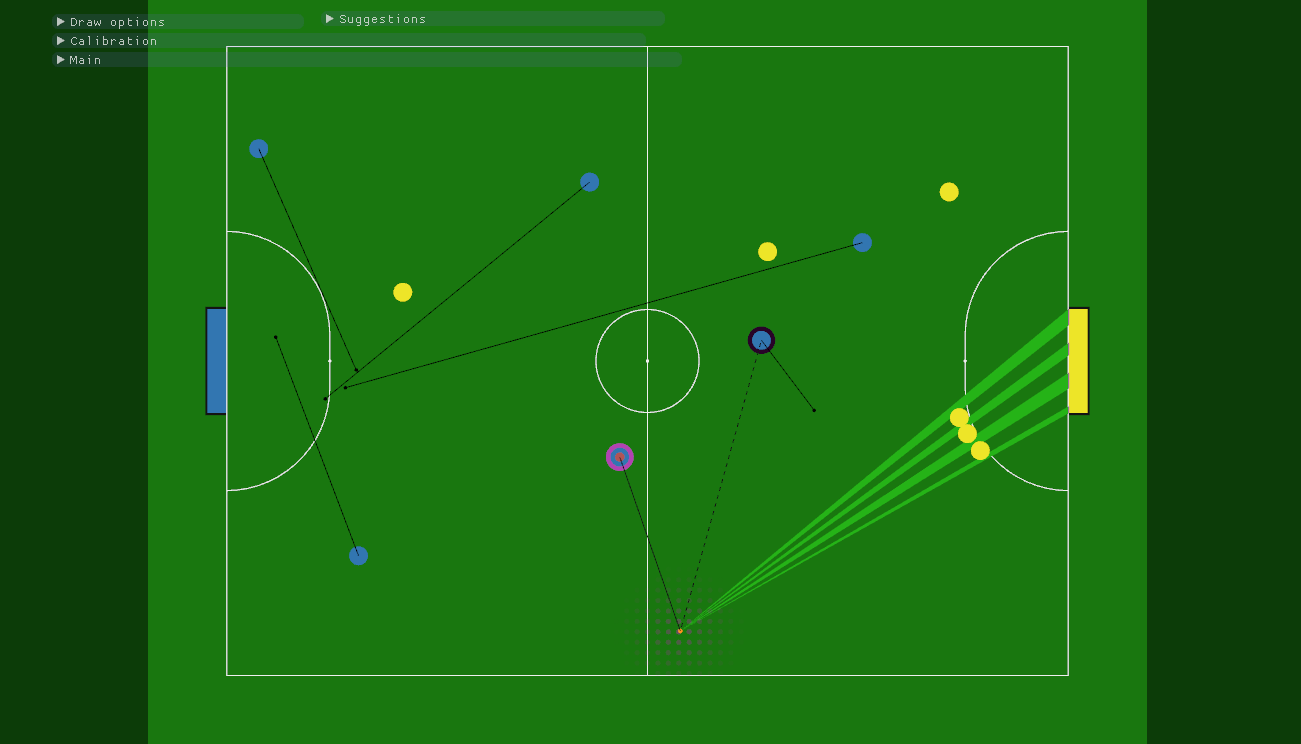
\includegraphics[width= 0.8\linewidth]{result/atack_atq_5000}
  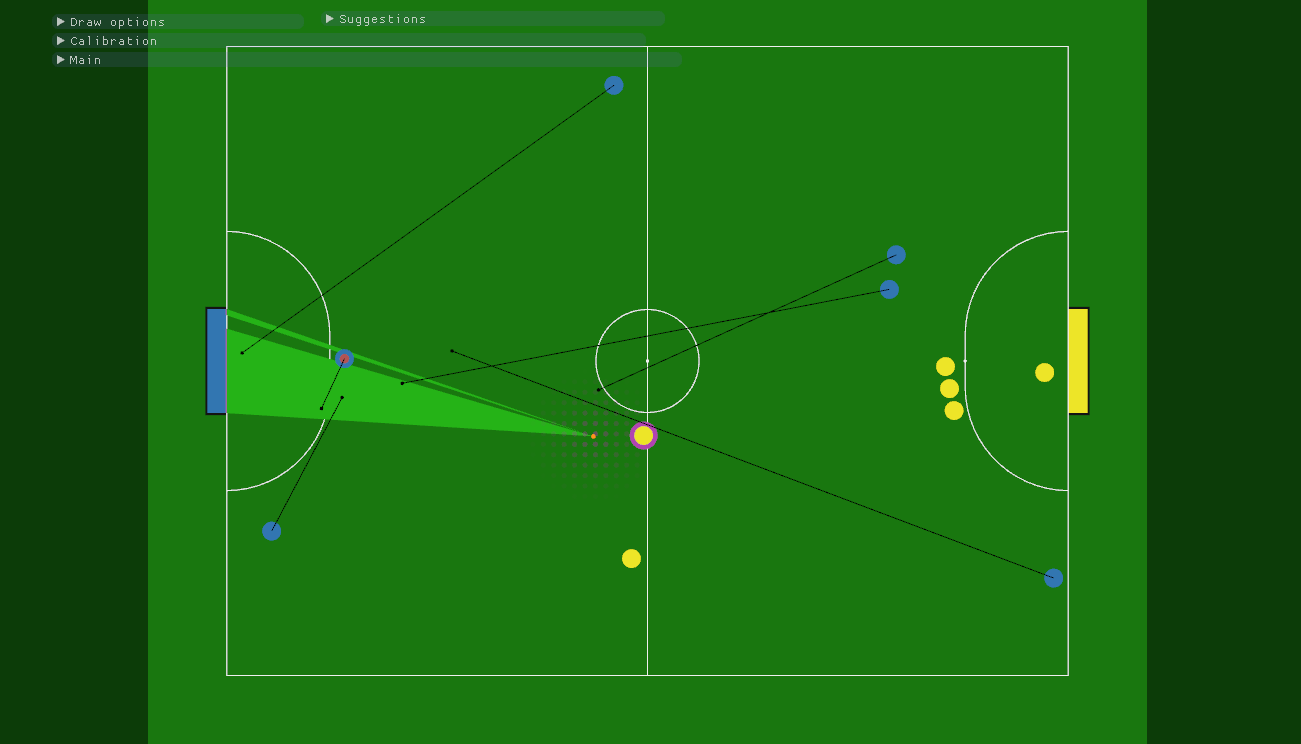
\includegraphics[width= 0.8\linewidth]{result/atack_def_5000}
  \caption{Planejamento com os parâmetros iniciais e o peso do custo do ataque
  alterado para $5000$.  No ataque (acima) e na defesa (abaixo)}\label{fig:atack_5000}
\end{figure}

% vim: tw=80 et ts=2 sw=2 sts=2 ft=tex
